\section{\uppercase{Results}}
\label{sec:results}
\noindent The forex market is a 24 hours market which main activity is
dominated by three major trading centers: Tokyo, London and New York. The seven
most important exchange rates are: the Australian Dollar (AUD), the Canadian
Dollar (CAD), the Swiss Franc (CHF), the British Pound Sterling (GBP),the Euro
(EUR), the Japanese Yen (JPY) and the Swedish Krona (SEK)~\cite{HaugetAl2000}.
Most HFT trades are done in those currencies, but increasingly New Zeland (NZD)
and Mexican Peso (MXN) have being automated traded.

Tests of OVECM were carried out using some of the main foreign exchange rates:
EURUSD, GBPUSD, USDCHF, USDJPY ~\cite{Dukascopy2014}. The reciprocal of the last
two rates (CHFUSD, JPYUSD) were used in order to obtain the same base currency
for all rates.  The tests were done using 1-minute frequency data from ask
prices which corresponded to 373.503 data points excluding flat weekends and
holidays from the 12th of August 2013 to the 12th of August 2014.

In estimating the VECM, we firstly checked for unit roots performing the
Augmented Dickey Fuller (ADF) test on the variables in levels and first
differences.

Table~\ref{tab:adf} shows that all currency rates cannot reject the unit root
test but they rejected it with their first differences. This means that all of
them are I(1) time series and we are allowed to use VECM and OVECM.


\begin{table}[h!]
\caption{Unit roots tests}
\label{tab:adf}
\begin{center}
\begin{tabular}{|l|c|c|c|c|c|}
\hline
& \textbf{Statistic} & \textbf{Critical value} & \textbf{Result}\\
\hline
EURUSD          & -0.64 & -1.94 & True       \\
$\Delta$ EURUSD & -70.45   & -1.94 & False       \\
GBPUSD          & -0.63   & -1.94 & True          \\
$\Delta$ GBPUSD & -54.53   & -1.94 & False       \\
CHFUSD          & -0.88   & -1.94 & True         \\
$\Delta$ CHFUSD & -98.98   & -1.94 & False       \\
JPYUSD          & -0.65 & -1.94 & True        \\
$\Delta$ JPYUSD & -85.78 & -1.94 & False     \\ 
\hline
\end{tabular}
\end{center}
\end{table}


\subsection{Setting parameters}

In order to set VECM parameter: $L$ and $p$, we use the Akaike Information
Criterion (AIC). RR parameter $\lambda$ was done by cross-validation.

\begin{figure}[h!]
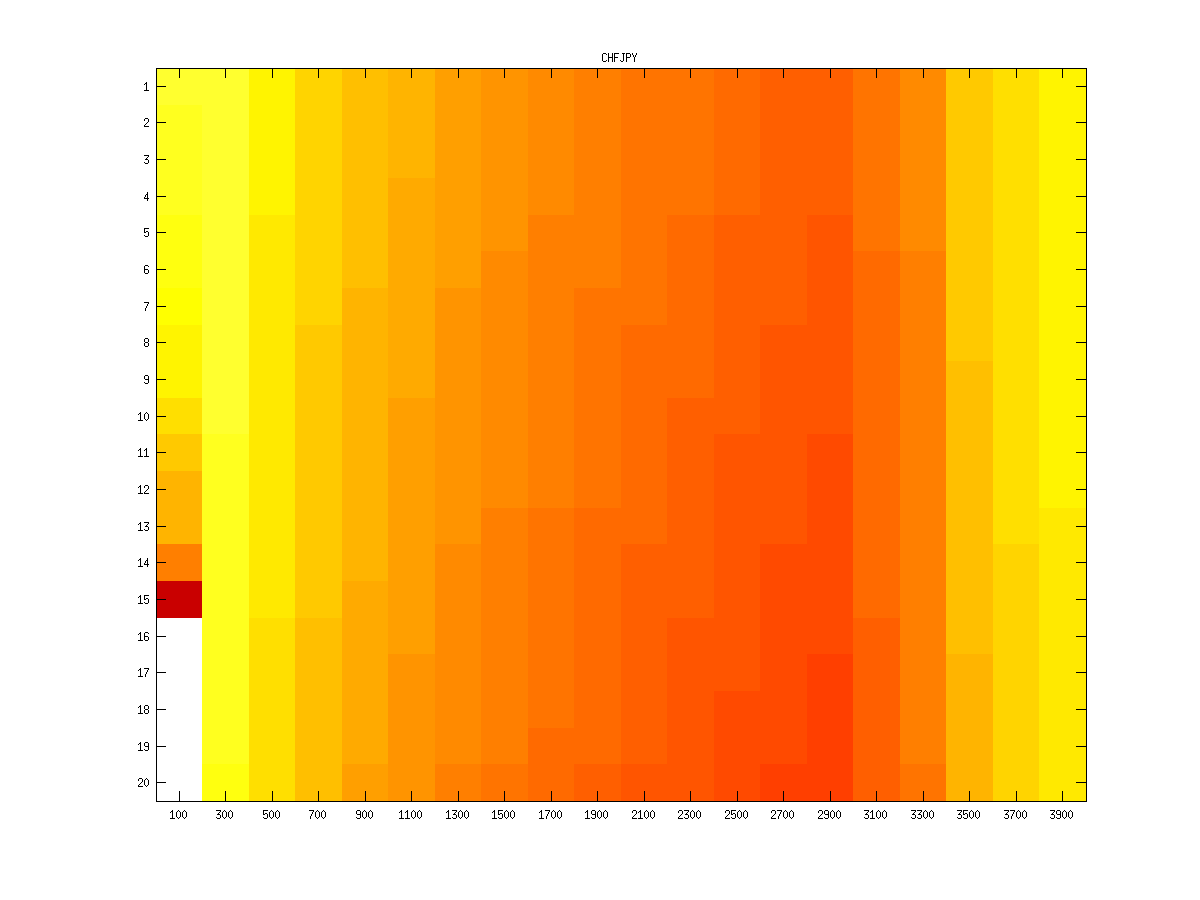
\includegraphics[width=0.5\linewidth]{img/vecm-params}
\caption{Setting VECM parameters}
\label{fig:shrinks}
\end{figure}

We ran OVECM and SLVECM 10.000 iterations for different values of sliding
window size $L$, number of lags $p$ and mean\_error (the latest only appliesto
OVECM). The execution times are shown in the table~\ref{tab:extimes}.

\begin{table}[h!]
\caption{Execution times}
\label{tab:extimes}
\begin{center}
\begin{tabular}{|l|c|c|c|c|c|}
\hline
& \textbf{L} & \textbf{P} & \textbf{mean\_error}  & \textbf{Time} \\
\hline
SLVECM & 300 & 4  & -- & 144\\
OVECM & 300 & 4  & 0 & 98\\
OVECM & 300 & 4  & 120 & 78\\
\hline
SLVECM & 300 & 8  & -- & 298\\
OVECM & 300 & 8  & 0 & 196\\
OVECM & 300 & 8  & 120 & 177\\
\hline
SLVECM & 3000 & 4  & -- & 324\\
OVECM & 3000 & 4  & 0 & 241\\
OVECM & 3000 & 4  & 120 & 97\\
\hline
SLVECM & 3000 & 8  & -- & 860\\
OVECM & 3000 & 8  & 0 & 632\\
OVECM & 3000 & 8  & 120 & 303\\
\hline
\end{tabular}
\end{center}
\end{table}

It is clear that execution time depends directly on $L$ and $p$ since they
determine the size of matrix $\mathbf{A}$ and therefore affect the OLS function
execution time.
It is worthy of note that execution time also depends on mean\_error because it
determines how many times OVECM will recalculate cointegration vectors which is
an expensive routine. Also, our proposal reduces execution time more than  50\%
in some cases.

Figure~\ref{fig:mapes} shows an example of the
in-sample MAPE. In consequence, OVECM performance increases when
mean\_error increases, but it will affect accuracy. Table~\ref{tab:mapes} shows
differents MAPEs out-of-sample for SLVECM and OVECM and all of them are very
similar. This supports the theory that cointegration vectors little with time.

\begin{table*}[ht!]
\caption{Out-of-sample MAPEs}
\label{tab:mapes}
\begin{center}
\begin{tabular}{|l|c|c|c|c|c|c|c|}
\hline
Method & \textbf{L} & \textbf{P} & \textbf{mean}  & \textbf{MAPE} & \textbf{MAPE}& \textbf{MAPE}& \textbf{MAPE}\\
&  &  & \textbf{error}  & \textbf{EURUSD} & \textbf{GBPUSD}& \textbf{CHFUSD}& \textbf{JPYUSD}\\
\hline
 SLVECM &   L=300 &  P=4&    &  134.76&  136.50&  133.16&  137.20\\
 OVECM  &   L=300 &  P=4& 0  &  134.76&  136.50&  133.16&  137.20\\
 OVECM  &   L=300 &  P=4& 120&  134.30&  135.53&  132.88&  136.44\\
\hline
 SLVECM &   L=300 &  P=8&    &  157.76&  160.55&  155.24&  162.74\\
 OVECM  &   L=300 &  P=8& 0  &  157.76&  160.55&  155.24&  162.74\\
 OVECM  &   L=300 &  P=8& 120&  158.03&  160.89&  155.30&  162.61\\
\hline
 SLVECM &   L=3000&  P=4&    &  111.91&  110.60&  109.22&  105.69\\
 OVECM  &   L=3000&  P=4& 0  &  111.91&  110.60&  109.22&  105.69\\
 OVECM  &   L=3000&  P=4& 120&  112.49&  111.26&  109.25&  105.88\\
\hline
 SLVECM &   L=3000&  P=8&    &  118.96&  118.97&  114.99&  110.57\\
 OVECM  &   L=3000&  P=8& 0  &  118.96&  118.97&  114.99&  110.57\\
 OVECM  &   L=3000&  P=8& 120&  119.23&  119.05&  114.82&  110.58\\
\hline
\end{tabular}
\end{center}
\end{table*}


% SLVECM    L=300   P=4             [ 134.7630329035  136.5086625175  133.1658744763  137.2084992162]
% SLVECM    L=300   P=8             [ 157.761485001   160.5552885679  155.2402883372  162.7438222296]
% SLVECM    L=3000  P=4             [ 111.91007246    110.6026357988  109.2219354574  105.6932468374]
% SLVECM    L=3000  P=8             [ 118.9663817354  118.9770962212  114.9939599829  110.5712975915]
% OVECM     L=300   P=4 AVGE=0      [ 134.7630329035  136.5086625175  133.1658744763  137.2084992162]
% OVECM     L=300   P=8 AVGE=0      [ 157.761485001   160.5552885679  155.2402883372  162.7438222296]
% OVECM     L=3000  P=4 AVGE=0      [ 111.91007246    110.6026357988  109.2219354574  105.6932468374]
% OVECM     L=3000  P=8 AVGE=0      [ 118.9663817354  118.9770962212  114.9939599829  110.5712975915]
% OVECM     L=300   P=4 AVGE=120    [ 134.301881303   135.5315795893  132.8835616177  136.4493817757]
% OVECM     L=300   P=8 AVGE=120    [ 158.0383643503  160.8908753314  155.3006014391  162.6119716451]
% OVECM     L=3000  P=4 AVGE=120    [ 112.4957023005  111.2666209761  109.2525274819  105.8804205046]
% OVECM     L=3000  P=8 AVGE=120    [ 119.2383924719  119.0508650247  114.8288372278  110.5815700448]


%\begin{figure}[!h]
%  \vspace{-0.2cm}
%  \centering
%   {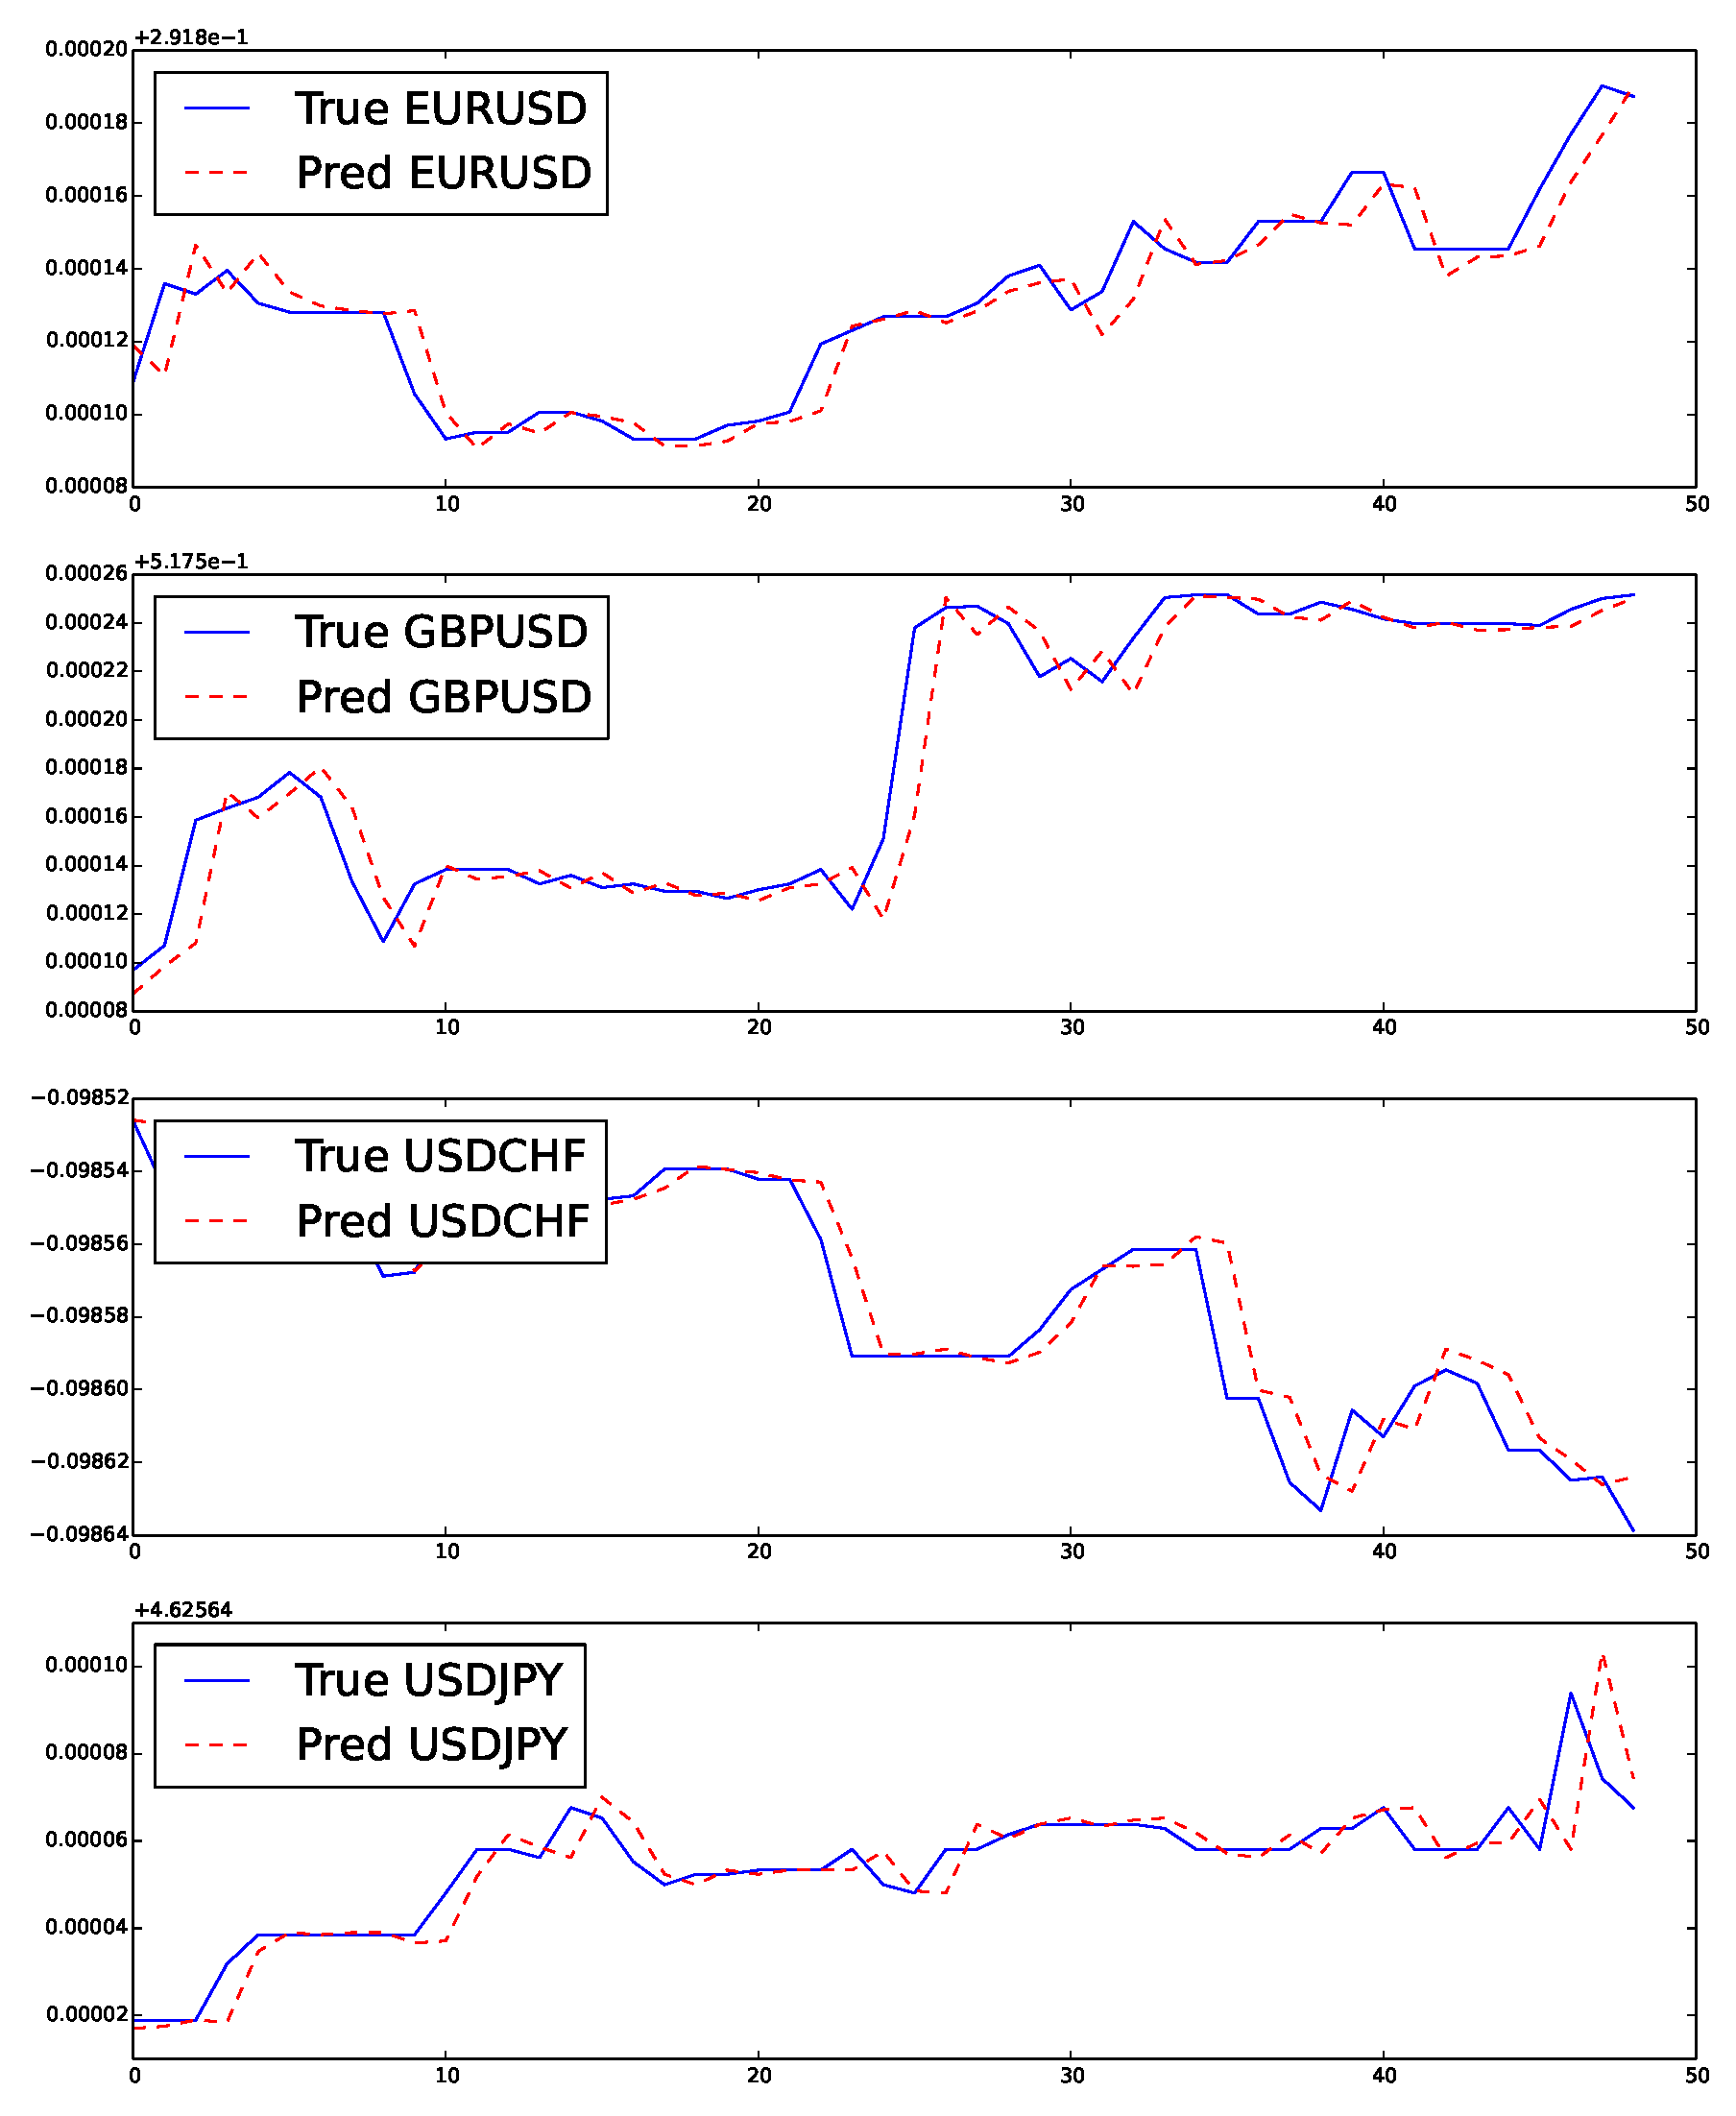
\epsfig{file = img/accuracy.eps, width = 7.5cm}}
%  \caption{Time series differences accuracy.}
%  \label{fig:accuracy}
% \end{figure}
%
%\begin{figure}[!h]
%  \vspace{-0.2cm}
%  \centering
%   {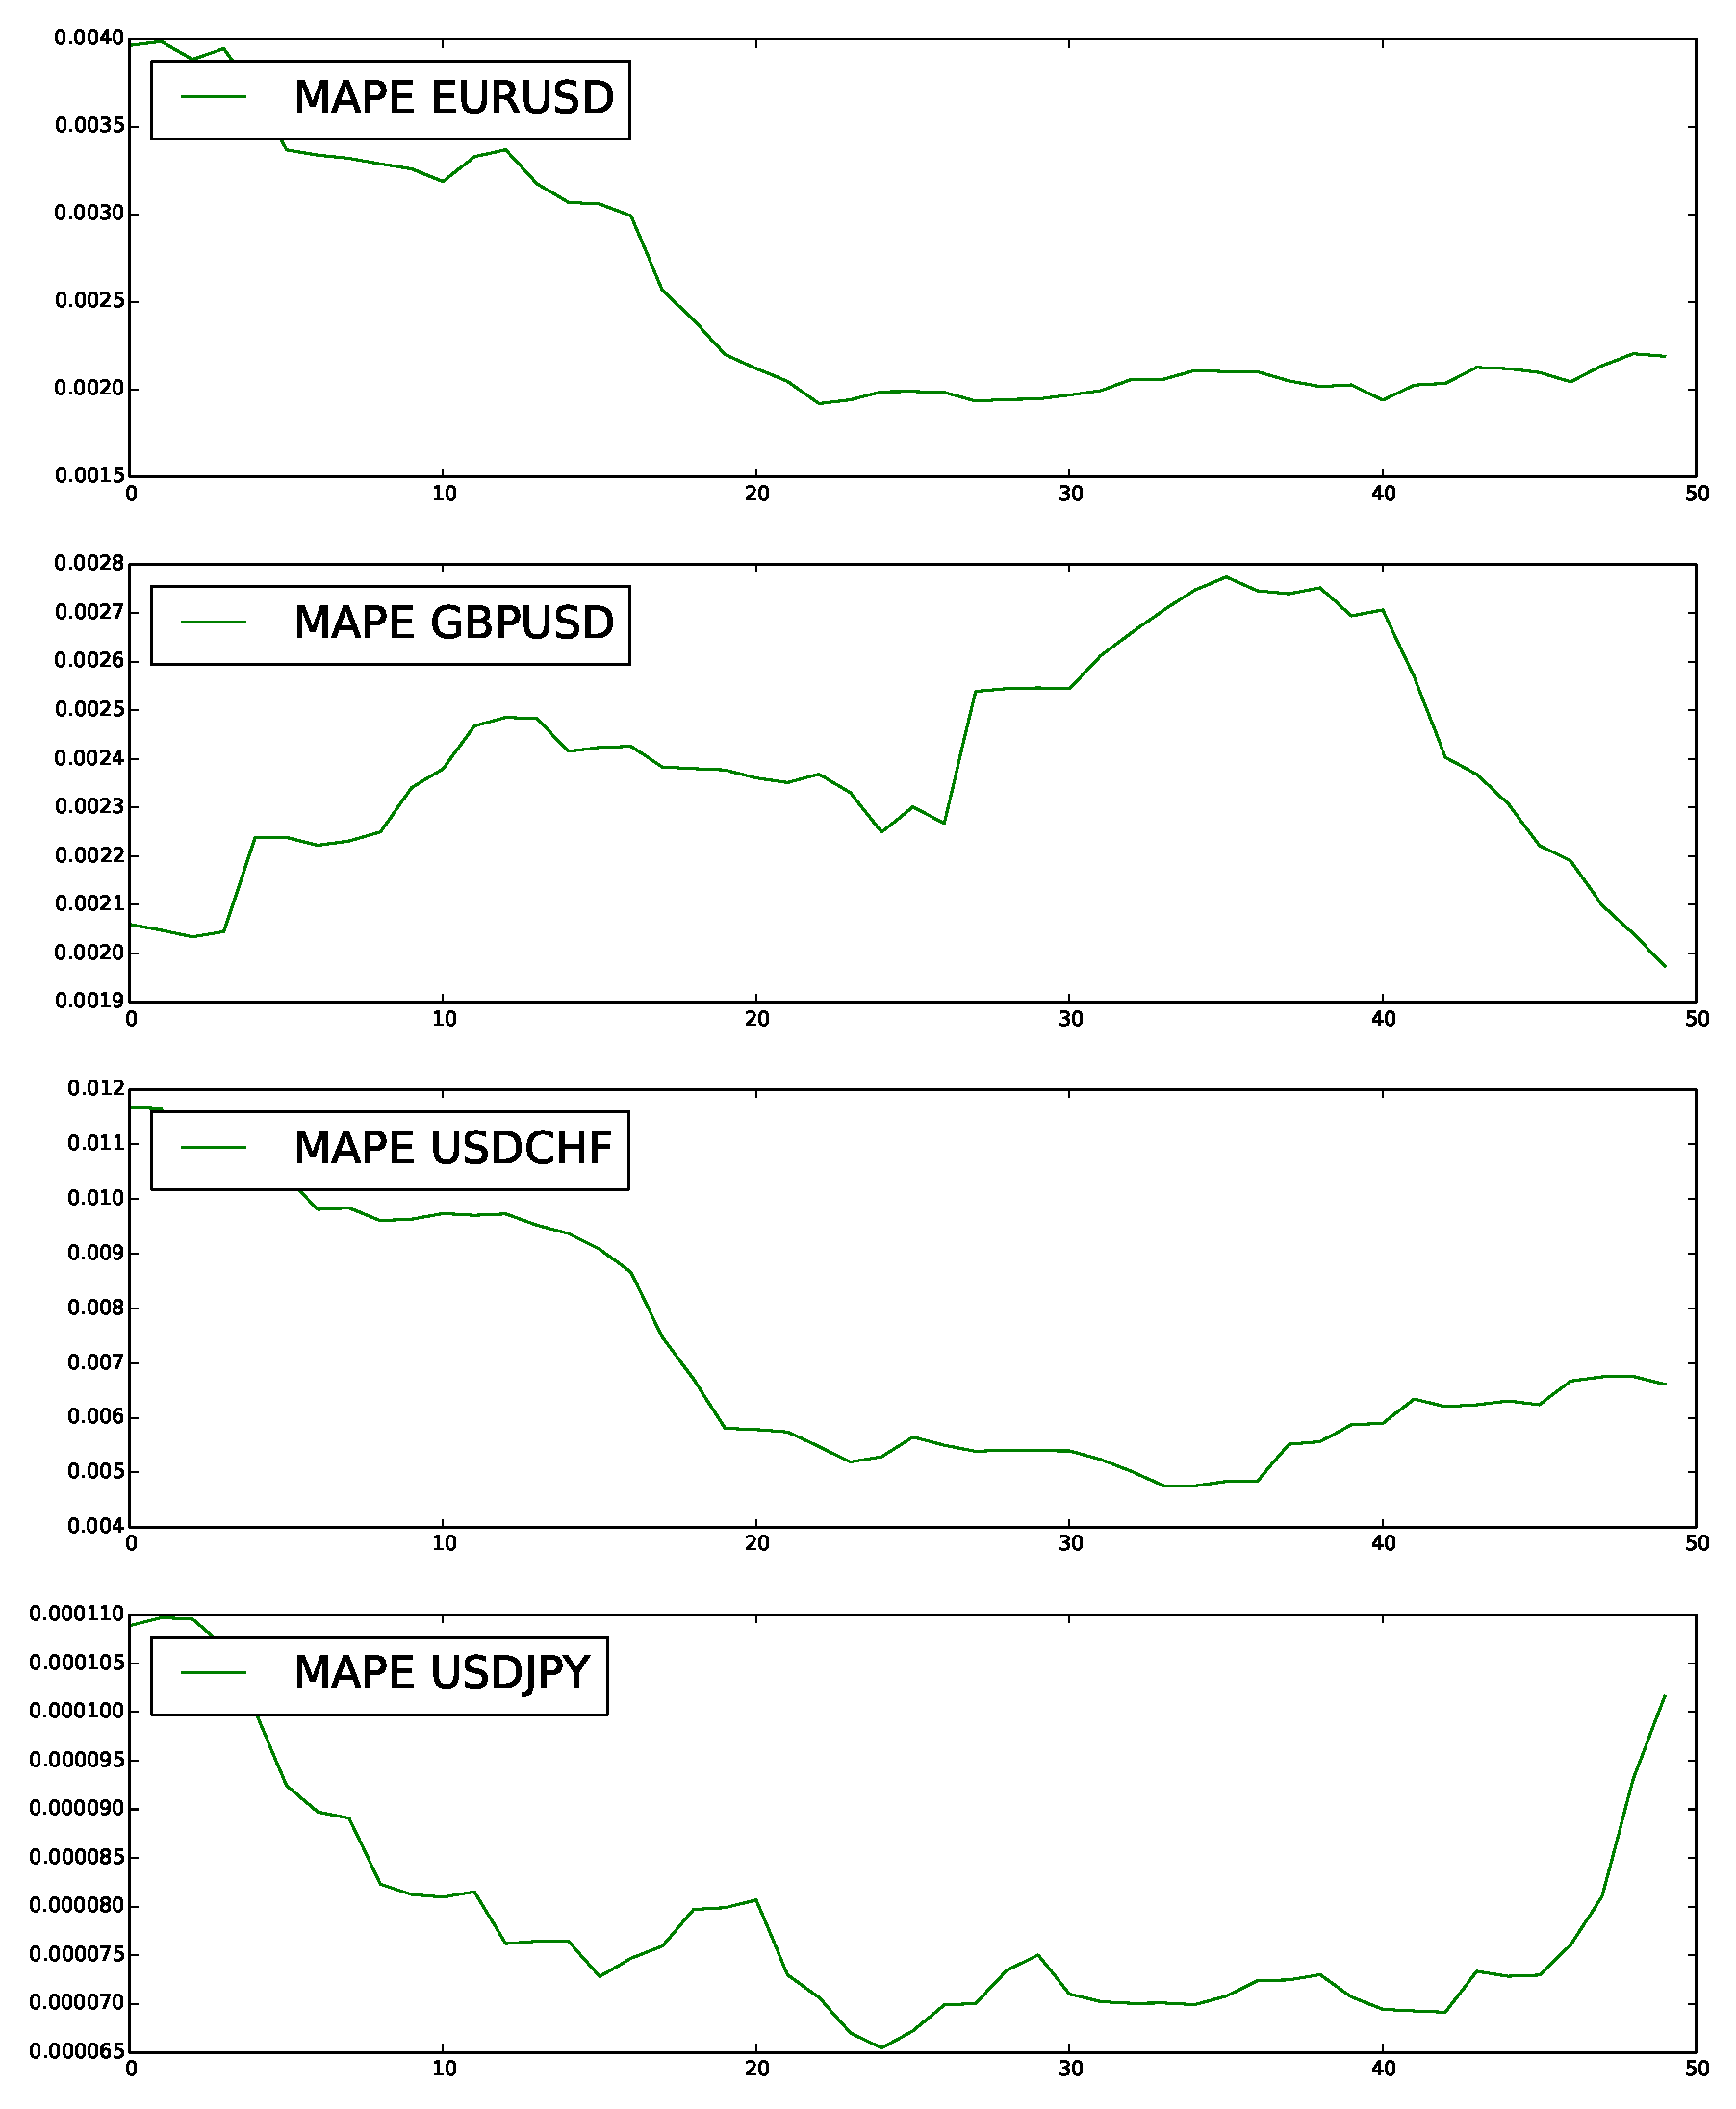
\epsfig{file = img/mapes.eps, width = 7.5cm}}
%  \caption{In-sample MAPEs example.}
%  \label{fig:mapes}
% \end{figure}

Despite the fact that MAPEs are high, figure ~\ref{fig:accuracy} shows some of
the out-of-sample forecasts made by our proposal OVECM which appears to follow
time series differences. 

